% Chapter 2

\chapter{Trasfondo del aprendizaje profundo} % Main chapter title

\label{Chapter2} % For referencing the chapter elsewhere, use \ref{Chapter1} 

En este capítulo se planteará y se explicará la base teórica del campo del aprendizaje profundo utilizados en este trabajo. Los conceptos descritos a continuación son el fundamento del campo de aprendizaje profundo


\section{Aprendizaje supervisado}

En el área de aprendizaje de máquina (profundo) existen dos tipos básicos de problemas. El tipo se determina dependiendo de el tipo de datos a utilizar para el entrenamiento del modelo.

Cuando los datos --- ya sea información tabulada, imágenes, textos --- no tienen ninguna categoría o ningún valor a predecir y lo que se desea es obtener información no específica, es decir sin tener alguna referencia, se trata de un aprendizaje no supervisado.

Si los datos, por otro lado, tengan una clasificación, llamada etiqueta, asignada, la cual a futuro es el resultado a predecir, los métodos a utilizar son los del aprendizaje supervisado. Debido a que el problema a abordar en este trabajo es un problema de clasificación, el resto del fundamento teórico será basado en el contexto del aprendizaje supervisado.

El aprendizaje supervisado puede entonces ser descrito como una función $f : X \to Y$ donde $X$ representa los datos con los que se alimenta la función, es decir con los que se entrenará el modelo, y $Y$ el resultado a asignado o a predecir.

Para ilustrar el proceso de aprendizaje de máquina profundo se utilizará un caso individual de la función en donde $y$ es el resultado deseado y $f(x) = \hat{y}$ es la función aplicada a un caso específico y $\hat{y}$ representa el resultado obtenido con la función el cual no necesariamente es el resultado deseado y esperado.

\textbf{El objetivo.} En concreto, buscamos una función $f$ que sea la mejor candidata para poder predecir los resultados deseados. Si definimos una función de costo $L(\hat{y}, y)$ que representa, en un valor escalar, la diferencia cuantitativa entre la evaluación de una función $f$ candidata y el resultado real $y$ podemos concluir que el objetivo es encontrar una $f^*$ que cumpla con:

$$f^* = \min_{f \in F} \frac{1}{N} \sum_{i = 0}^{N} L(f(x_i), y_i)$$

Donde $n$ es el número de instancias de los datos para entrenar el modelo; $F$ siendo un conjunto de funciones candidatas.

\textbf{Definiendo las funciones.} La base de todo modelo de aprendizaje profundo es una red neuronal --- cuyo comportamiento será definido en la siguiente sección junto con otros detalles --- y su comportamiento puede ser descrito de la siguiente forma:

$$ f(x_i) = w x_i + b $$

Siendo $x_i$ la instancia $i$ con propósitos de entreno o de predicción. Esto nos dice que $w$ y $b$ serán los parámetros a modificar de una manera sistemática para encontrar la función $f^*$. Con fines de brevedad, la concatenación de $w$ y $b$ serán representados por $\theta$.

La función de pérdida para una predicción obtenida toma la forma del error de la entropía cruzada, es decir:

$$ L(\hat{y_i}, y_i) = y_i log\hat{y_i} + (1 - y_i)log(1 - \hat{y_i}) $$

Teniendo ya la pérdida para una predicción se puede expandir esta idea para obtener la pérdida a través de un conjunto de datos, lo cual resultará muy útil cuando se deba entrenar. Para obtener una aproximación de la perdida sobre un conjunto de datos se podrá utilizar el promedio sobre las perdidas individuales de los datos evaluados:

$$ L(\hat{y}, y) = - \frac{1}{N} \sum_{i = 1}^{N} [y_i log\hat{y_i} + (1 - y_i)log(1 - \hat{y_i})] $$

\textbf{Optimizando la función de costo.} Teniendo entonces una función a minimizar y una cantidad $N$ de datos sobre los cuales se deberá ir encontrando una función $f$ candidata cada vez mejor se recurre al método de el descenso de gradiente. Este método nos permite, utilizando propiedades básicas de las derivadas de las funciones, poco a poco avanzar hasta llegar a un mínimo de la función. Cada nueva función candidata entonces podrá ser derivada de la siguiente forma:

$$ f_i(x_i) = \theta_i x_i $$

Donde

$$ \theta_{i + 1} = \theta_{i} - \gamma \nabla L(\hat{y_i}, y_i) $$

Este proceso de utilizar el descenso de gradiente a través de las instancias nos permite ir minimizando el error de la función hasta poder deducir la función que muestra el menor error.

\textbf{La tasa de aprendizaje.} La velocidad de convergencia de este proceso dependerá en gran parte en $\gamma$ que representa la tasa de aprendizaje, es decir, es la ponderación que se le da al gradiente cuando se propone la nueva función. Un $\gamma$ muy alto arriesga una divergencia debido a que podría oscilar alrededor de un mínimo sin nunca poder converger en él. Un $\gamma$ muy bajo, por el otro lado, puede resultar en un aprendizaje muy lento, lo cual puede llevar a un resultado no óptimo. Este concepto será importante en capítulos posteriores de este trabajo.

\section{Redes neuronales}

Las redes neuronales son el modelo base para el aprendizaje profundo. Con ayuda de el concepto de las redes neuronales especificaremos más acerca de la función $f$ que hasta ahora ha permanecido general, únicamente sabiendo que es derivable. Hay diferentes tipos de redes neurales en el campo y en este trabajo se abordarán únicamente las redes neuronales estándar y las recurrentes.

\subsection{Redes neuronales estándar}

\begin{figure}
	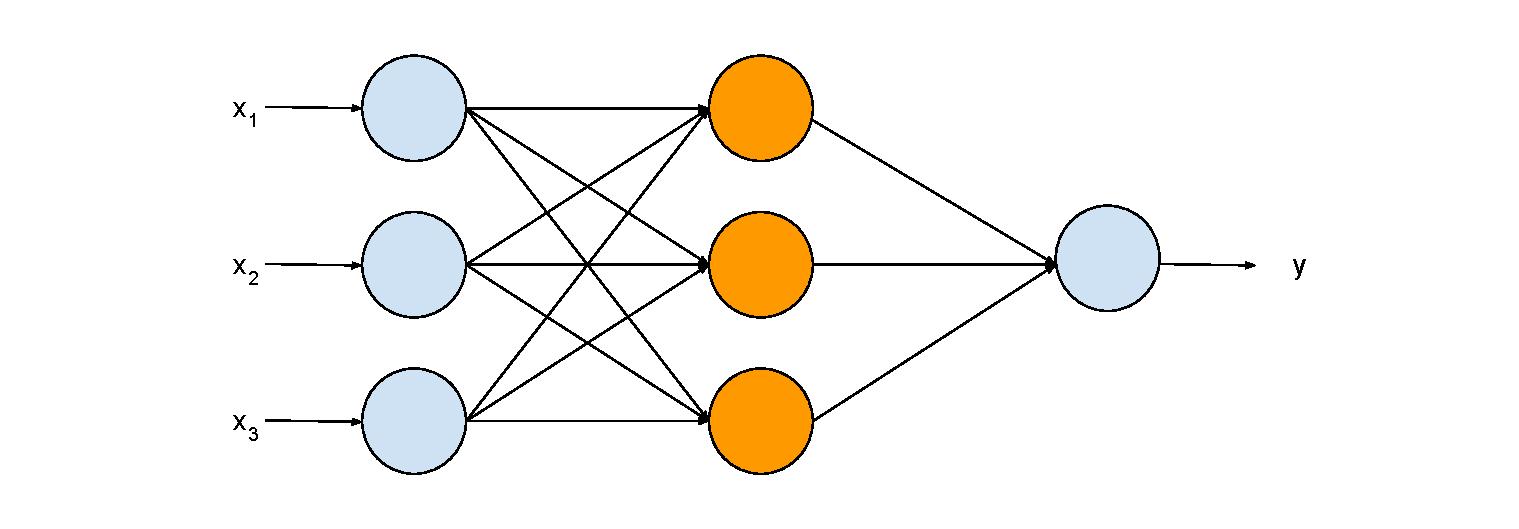
\includegraphics[scale=.6]{Figures/standardnn.pdf}
	\caption{Una red neuronal estándar con una capa oculta, la cual tiene 3 unidades neuronales. La red está completamente conectada y tiene 3 nodos de entrada.}
	\label{fig:standardnn}
\end{figure}

\textbf{Inspiración.} Estas redes neuronales fueron basadas en comportamientos biológicos y reflejan un comportamiento similar a la comunicación de neuronas que se aprecia en la naturaleza. La entrada de datos en una neurona es procesada y alimentará a la siguiente neurona y así sucesivamente hasta haber recorrido toda la red. La redes neuronales no son sucesiones directas y lineales de neuronas; las redes están divididas en capas, las cuales pueden contener más de una unidad. En una red completamente interconecteda, como la que se aprecia en la figura \ref{fig:standardnn}, conecta a todas las unidades de una capa con todas las unidades de la siguiente.

\subsection{Redes neuronales recurrentes}